\section{Kommunikation}
Die Kommunikation der App mit dem Server läuft bei der Kommunikation der App mit dem RESTful Webservice über Http befehle und für das Senden von Alarmnachrichten an die verschiedenen Geräte  wird Google Cloud Messaging verwendet.
\subsection*{Google Cloud Messaging}
Der Service Google Cloud Messaging (GCM) wird Entwicklern von Android Apps kostenlos von Google zur Verfügung gestellt. Er erlaubt diesen über bestehende Google Server Infrastruktur Daten an ihre Apps  und von diesen an ihren Server zu senden. Hierbei übernimmt der GCM Service alle aufgaben die mit der Übermittlung  der Nachricht zu tun haben.\\

Hier eine Auflistung der Hauptfunktionen von GCM:

\begin{itemize}
	\item Senden von Nachrichten vom Eigenen Server zu den Nutzergeräten
	\item Empfangen von Nachrichten der Nutzergeräte am Server
	\item Die App muss nicht laufen um Nachrichten zu empfangen
	\item Es gibt keine Grafische Oberfläche sämtliche Aufgaben die mit der Nachricht zusammenhängen werden von der eigenen Anwendung gesteuert.
	\item Voraussetzung ist Android 2.2 Froyo mit Installiertem Playstore
\end{itemize}

\subsubsection*{Architektur}
Die Architektur von Google Cloud Messaging  teilt sich in drei Bereiche auf der erste sind die GCM Connection Server die die Nachrichten von den Servern des Entwicklers annehmen und dieses an die Android App des Benutzers schicken. Der zweite Bereich ist der Server des Entwicklers der die Nachrichten für die Benutzer Apps an die Connection Server sendet und als dritten Bereich natürlich die Benutzer-App die sich zum Empfang von GCM Nachrichten bei GCM Registrieren muss um eine eindeutige ID zu erhalten und dadurch nur für sie bestimmte  Nachrichten zu erhalten.\\

\begin{figure}[H]
\centering
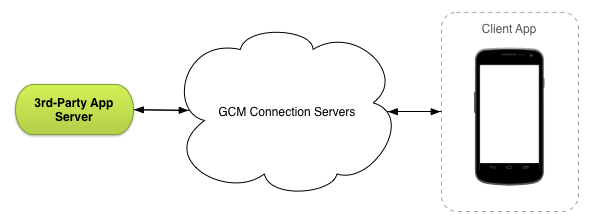
\includegraphics[width=\textwidth]{/GCMstruktur.png}
\caption{Struktur von GCM}
\label{fig:GCMstrukutr}
\end{figure}

\subsubsection*{Android}
Das Empfangen von Nachrichten in der App läuft über das Packet GcmIntentService.java hier werden die Empfangenen Nachrichten nach ihrem Typ sortiert bei dem Messagetyp Send error wird der Fehler als solcher Makiert ins Log geschrieben. Bei dem Messagetyp Deleted wird nach demselben Prinzip vorgegangen. Beim Typ Message wird die Prozedur NotificationsService.sendAlarmNotification aufgerufen. Hierdurch werden in Android die Notifications ausgelöst.\\

\begin{lstlisting}[caption={Empfangen von GCM Nachrichten unter Android},label=lst:GCMget]

    @Override
    protected void onHandleIntent(Intent intent) {
        Bundle extras = intent.getExtras();
        GoogleCloudMessaging gcm = GoogleCloudMessaging.getInstance(this);
        String messageType = gcm.getMessageType(intent);

        if (!extras.isEmpty()) {

            if (GoogleCloudMessaging.MESSAGE_TYPE_SEND_ERROR.equals(messageType)) {
            		Log.i(TAG, "Send error: " + extras.toString());
	            }
 	else if (GoogleCloudMessaging.MESSAGE_TYPE_DELETED.equals(messageType)) {
            		Log.i(TAG,  "Deleted messages on server: " + extras.toString());
            	}
	else if (GoogleCloudMessaging.MESSAGE_TYPE_MESSAGE.equals(messageType)) {
            		NotificationsService.sendAlarmNotification(this, extras.getString("message"));
                	Log.i(TAG, "Received: " + extras.toString());
            	}
        	}
        GcmBroadcastReceiver.completeWakefulIntent(intent);
	} 
}

\end{lstlisting}

\subsubsection*{Server}
Der Server sendet \ref{ServerSeGCM} eine Benachrichtigungen an die GCM Server diese Leiten die Nachricht an die betroffenen Geräte-IDs weiter. Dies wird über einen REST-Methodenaufruf durchgeführt. Dieser wird an die Adresse https://android.googleapis.com/gcm/send gesendet die Nachricht ist mit einem Authorisationskey ausgestattet damit nur Nachrichten vom richtigen Server gesendet werden können 

\begin{lstlisting}[caption={Senden von Nachrichten vom Server},label=lst:ServerSeGCM]

URL url = new URL(this.configuration.getApiUrl());
			HttpURLConnection http = (HttpURLConnection) url.openConnection();
			http.setDoOutput(true);
			http.setRequestMethod("POST");
			http.setRequestProperty("Content-Type", "application/json");
			http.setRequestProperty("Authorization", "key="+this.configuration.getAuthorizationKey()); //
			
			OutputStreamWriter writer = new OutputStreamWriter(http.getOutputStream());
			writer.write(rawData.toString());
			writer.flush();

\end{lstlisting}

Der Server empfängt \ref{lst:ServerEmGCM} auserdem eine bestätigung der Zustellung von den GCM Servern diese enthält eine Zahl die koodiert ob die Nachricht angekommen und richtig interpretiert wurde. Bei Erfolg wird die Nachricht mit Code 200 bestätigt. Bei einer JSON Nachricht kann auch der Code 400 gesendet werden wenn z.B. ein anderer Datentyp als erwartet gesendet wurde. Wenn der Code 401 gesendet wird, ist die Authentifizierung am GCM Server nicht mit Erfolg abgeschlossen worden. hiermit wird sichergestellt das Nachrichten nur vom richtigen Server gesendet werden können. 


\begin{lstlisting}[caption={Empfangen von Bestätigungen am Server},label=lst:ServerEmGCM]

BufferedReader reader = new BufferedReader(new InputStreamReader(http.getInputStream()));
			StringBuilder result = new StringBuilder();
			
			for (String line; (line = reader.readLine()) != null; ) {
				result.append(line);
			}

			writer.close();
			reader.close();

\end{lstlisting}
